%% ZETA-IoT — revised manuscript addressing IoT 2026 review (double-blind).
%% Compile on Overleaf: ACM Conference Proceedings "Master" Template
%% (acmart / sample-sigconf), replace files with this project.
\documentclass[sigconf,review,anonymous]{acmart}

%% ACM ICPS rights block placeholders (final values set after acceptance)
\setcopyright{acmlicensed}
\acmConference[IoT 2026]{16th International Conference on the Internet of Things}{November 17--20, 2026}{Newcastle upon Tyne, United Kingdom}
\acmBooktitle{16th International Conference on the Internet of Things (IoT 2026), November 17--20, 2026, Newcastle upon Tyne, United Kingdom}
\acmPrice{}
\acmISBN{}
\acmDOI{}

\usepackage{booktabs}

\begin{document}

\title{ZETA-IoT: A Zero-Trust Ensemble Architecture with Tiered AI Governance for Resource-Constrained IoT Edge Security}

\author{Anonymous Author(s)}
\affiliation{%
  \institution{Anonymous Institution}
  \city{}
  \country{}}
\email{anonymous@example.com}

\begin{abstract}
IoT devices at the network edge are hard to secure: they lack the resources for conventional security stacks, and the machine-learning defences that could protect them fall within the scope of governance frameworks such as the NIST AI RMF and the EU AI Act. This paper presents ZETA-IoT, a Zero-Trust Ensemble Architecture with Tiered AI Governance; its compliance layer \emph{maps} design elements onto AI RMF functions and AI Act articles, and we are explicit that this mapping is a design alignment, not a determination of legal applicability or compliance. Its four layers combine a hardware root of trust, zero-trust microsegmentation, a tiered AI governance engine that splits decisions between autonomous edge AI and human analysts by stakes and score severity, and the compliance layer itself. The detection layer, three lightweight detectors (Isolation Forest, one-class SVM, autoencoder) trained only on benign traffic, is evaluated on N-BaIoT, real traffic from nine commercial IoT devices infected with Mirai and BASHLITE. Window-level decisions catch 100\% of all ten attack types at a 1.45\% false-positive rate, macro-AUC 0.9996, from an ensemble averaging 3.6\,MB of serialized storage per device. That saturation is partly a property of the benchmark: margins above threshold vary by orders of magnitude, and the BASHLITE floods clear the alarm line by less than a factor of two, which is a more informative number than the headline rate. An ablation shows that score fusion can mask attacks that individual detectors catch, arguing for ensemble diversity as a design requirement rather than a tuning choice. The evaluation protocol is specified exactly, including its non-chronological nature; a chronological held-out check on the largest benign capture shows the benign false-positive rate does not degrade under temporal ordering. The governance engine routes these real anomaly scores across decision tiers under an explicit, complete decision contract, and a 14-indicator Security Performance Indicator framework is proposed, reporting what is measurable without a live deployment and deferring the rest honestly. Code and evaluation artefacts are available in an anonymized artifact repository (\url{https://anonymous.4open.science/r/zeta-iot-artifact-42B3}).
\end{abstract}

\begin{CCSXML}
<ccs2012>
<concept>
<concept_id>10002978.10002991.10002995</concept_id>
<concept_desc>Security and privacy~Network security</concept_desc>
<concept_significance>500</concept_significance>
</concept>
<concept>
<concept_id>10010520.10010553.10010562</concept_id>
<concept_desc>Computer systems organization~Embedded and cyber-physical systems</concept_desc>
<concept_significance>300</concept_significance>
</concept>
<concept>
<concept_id>10010147.10010257</concept_id>
<concept_desc>Computing methodologies~Machine learning</concept_desc>
<concept_significance>300</concept_significance>
</concept>
</ccs2012>
\end{CCSXML}
\ccsdesc[500]{Security and privacy~Network security}
\ccsdesc[300]{Computer systems organization~Embedded and cyber-physical systems}
\ccsdesc[300]{Computing methodologies~Machine learning}

\keywords{IoT security, zero-trust architecture, AI governance, anomaly detection, edge computing, NIST AI RMF, EU AI Act, N-BaIoT}

\maketitle

\section{Introduction}
\label{sec:introduction}

By 2025 there were an estimated 21.1 billion connected IoT devices worldwide, with forecasts still pointing to double-digit growth through 2030~\cite{iotanalytics2025}. Much of modern infrastructure now sits on top of them: building automation, factories, hospitals, energy networks. Defences have not kept pace. When researchers dissected the Mirai botnet, they found that nothing more sophisticated than default passwords and stale firmware had handed hundreds of thousands of consumer devices to attackers, enough to mount record-breaking DDoS campaigns~\cite{antonakakis2017mirai}. Years later, insecure defaults still sit near the top of the OWASP IoT Top 10~\cite{owasp2018}.

Securing these devices runs into a structural tension. A camera or a smart thermostat cannot run a conventional security stack; its CPU, memory, and energy budgets are too small, and the gateway its traffic passes through is usually not much better off. The defences that do scale to this setting increasingly rely on machine learning, and that raises a second problem, because ML-based security functions deployed in critical infrastructure sit within the scope of AI governance frameworks. The NIST AI Risk Management Framework~\cite{nistairmf}---a voluntary framework~\cite{nistairmfvoluntary}---organises trustworthy-AI practice around four functions, and the EU AI Act~\cite{euaiact} makes human oversight and robustness legal requirements for high-risk systems (Articles 14 and 15). What neither says is how to provide that oversight when the decisions in question happen in milliseconds, at the network edge, far from any analyst's screen. A firewall rule can be reviewed at leisure; an autonomous quarantine decision on a hospital infusion pump cannot. Throughout this paper, mappings from ZETA-IoT mechanisms to these frameworks are \emph{design mappings}: engineering targets derived from the frameworks' requirements, not evidence that any legal obligation applies to a given deployment, and not a conformity assessment.

Zero-Trust Architecture~\cite{nist800207} answers the erosion of the network perimeter with a simple rule: never trust, always verify. Applying that rule across a heterogeneous IoT estate is far from simple, though, and remains an open problem~\cite{syed2022zta}. The literature has also tended to treat device security, network security, ML detection, and AI governance in isolation from one another.

\subsection{Research Gaps}

Three gaps stand out. The first is architectural fragmentation (G1): hardware trust, zero-trust networking, lightweight ML detection, and human governance each have their own literatures, but no unified architecture brings them together for resource-constrained environments. The second is a governance disconnect (G2): regulators ask for a human in the loop, yet no one has shown how that works when IoT security decisions take milliseconds. The third is validation realism (G3): detection schemes are routinely validated with attack samples already available at training time, which flatters their performance against attacks that are actually new. ZETA-IoT is designed to close all three gaps at once, through the contributions below.

\subsection{Contributions}

This paper makes four contributions:

\textbf{C1 --- ZETA-IoT architecture.} A four-layer design artefact that joins a hardware root of trust, zero-trust microsegmentation, a tiered AI governance engine, and a compliance layer into one coherent whole (Section~\ref{sec:arch}).

\textbf{C2 --- Tiered AI governance.} A three-tier decision taxonomy (autonomous, escalated, deferred) that maps directly onto NIST AI RMF functions and EU AI Act articles as design targets, giving human oversight an operational form in real-time IoT security, together with a complete decision contract covering every stakes/severity combination, override timeouts, and unavailable analysts (Section~\ref{sec:taige}).

\textbf{C3 --- Empirical validation of the detection layer.} A reproducible evaluation on the N-BaIoT benchmark~\cite{meidan2018nbaiot}, using real traffic from nine commercial IoT devices under Mirai and BASHLITE infection. Training sees benign traffic only, and the ensemble still detects 100\% of all ten attack types at window level, at a 1.45\% false-positive rate, within a mean 3.6\,MB serialized footprint per device (Section~\ref{sec:results}). A development ablation traces how fusion strategy and detector diversity decide whether flood attacks that fool individual detectors get caught, and the evaluation protocol is now specified to the operation order, including an explicit statement of its non-chronological nature and a chronological held-out check on the largest benign capture.

\textbf{C4 --- SPI framework and honest scoping.} A 14-indicator Security Performance Indicator framework covering detection, resilience, governance, and resources. Only the subset measurable from the dataset-based evaluation is reported; anything that needs a live deployment, such as human override rates, is deferred to a planned pilot instead of being estimated synthetically.

The empirical claims are deliberately scoped: Layers 1, 2, and 4 are presented as a design with concrete implementation paths on commodity components (TPM~2.0, eBPF/XDP, policy engines), while quantitative results in this paper concern Layer~3 detection and decision routing. This separation of validated results from design proposals is arguably a methodological contribution in itself, given documented concerns about validation realism in IoT security research~\cite{arp2022dodo}.

\section{Related Work}

\subsection{IoT Security and Botnet Detection}
Stankovic~\cite{stankovic2014} articulated security-by-design as a research direction for IoT; Granjal et al.~\cite{granjal2015} surveyed protocol-level security and identified persistent gaps between theoretical guarantees and deployment constraints, while Alrawais et al.~\cite{alrawais2017} examined security and privacy challenges when IoT workloads shift to fog and edge infrastructure. On the empirical side, Antonakakis et al.~\cite{antonakakis2017mirai} provided the definitive measurement study of Mirai, tracing hundreds of thousands of infections back to a handful of unchanged factory-default credentials. For detection, Meidan et al.~\cite{meidan2018nbaiot} introduced N-BaIoT, training per-device deep autoencoders \emph{exclusively on benign traffic} over the same 115 statistical traffic features used here, with benign data divided chronologically into training, optimization, and test sets, and released the dataset used in this paper. We adopt their benign-only, per-device evaluation philosophy; we state this plainly because an earlier version of this paper mistakenly claimed benign-only training as a point of difference. The present work differs from N-BaIoT in the detector design and its architectural context rather than in the training data policy: an ensemble of three complementary lightweight detectors chosen for divergent failure modes (rather than a single autoencoder family), an explicit threshold-margin analysis (Figure~\ref{fig:margins}), and embedding detection inside a governance architecture with a complete decision contract. We also correct an efficiency-related comparison: the N-BaIoT autoencoders are remarkably small (a 172\,kB object size per device, their Table~III), so the 3.6\,MB serialized ZETA-IoT ensemble is \emph{not} a smaller detector. Our resource claims are therefore restricted to what we measure---x86 scoring latency and serialized storage---and no model-size ranking against that work is claimed.

Diro and Chilamkurti~\cite{diro2018} demonstrated distributed deep-learning detection at fog nodes, reporting 99.14\% multiclass accuracy on NSL-KDD and 99.36\% binary accuracy on BoT-IoT with feed-forward and LSTM models trained on labelled attack traffic. Those numbers are not directly comparable to the results in Section~\ref{sec:results}: NSL-KDD is a general-purpose network intrusion benchmark from outside the IoT domain, and neither dataset involves traffic from genuinely compromised consumer devices in the way N-BaIoT does. The comparison is worth stating plainly, though, because it illustrates gap G3 from Section~\ref{sec:introduction} directly: a detector can look excellent on a benchmark built for a different threat model and still say little about a botnet-infected doorbell. Against this line, the present work differs by training exclusively on benign data rather than labelled attack traffic, by constraining the detector to commodity-CPU, megabyte-scale ensembles, and by embedding detection inside an explicit governance architecture rather than treating it as a standalone classifier.

\subsection{Zero Trust for IoT}
NIST SP~800-207~\cite{nist800207} formalises ZTA around a policy decision point that makes access decisions and a policy enforcement point that carries them out, with continuous evaluation replacing the one-time perimeter check. The model was written with enterprise networks in mind, where every asset can plausibly run an identity agent and phone home to a policy engine. Syed et al.~\cite{syed2022zta} survey ZTA comprehensively and identify IoT as the domain where that assumption breaks down hardest: constrained endpoints cannot run agents, cannot always reach a remote decision point within a useful time budget, and often cannot even hold a full TLS stack. Two responses to that gap dominate the literature. One pushes policy decisions into the cloud and accepts the round-trip latency; the other pushes them onto local infrastructure the IoT devices do not control, typically a gateway or edge router. ZETA-IoT's Layer~2 design takes the second path deliberately: enforcement sits at the gateway, uses kernel-level eBPF/XDP filtering, and consults trust scores that are pre-computed rather than fetched, so a policy decision never depends on a network round trip that a compromised or congested link could delay or deny.

\subsection{Adversarial Robustness of ML Detection}
ML-based intrusion detection is itself attackable. Alhajjar et al.~\cite{alhajjar2021} showed that evolutionary and GAN-based perturbations evade ML classifiers in network intrusion detection at high rates, and Arp et al.~\cite{arp2022dodo} catalogued pervasive methodological pitfalls in ML security research, including unrealistic threat models and data snooping. Two design choices in ZETA-IoT trace directly back to these findings. Training uses benign data only, since defenders rarely have samples of tomorrow's attack in advance. And the ensemble deliberately mixes detectors with different inductive biases, so that fooling one is not the same as fooling all three; Section~\ref{sec:ablation} states precisely what this fusion does and does not guarantee.

\subsection{AI Governance and Human Oversight}
On the governance side, the NIST AI RMF~\cite{nistairmf} organises trustworthy-AI practice around four functions (Govern, Map, Measure, Manage), while the EU AI Act~\cite{euaiact} makes human oversight and robustness legal requirements for high-risk systems (Articles 14 and 15). Whether a given deployment is high-risk depends on its context of use; the mapping in this paper assumes a deployment in which the system functions as a security-management component for network operations, and we map design elements to the Act's Articles 14--15 requirements as engineering targets only. The AI RMF, for its part, is explicitly voluntary~\cite{nistairmfvoluntary}. Neither document specifies an architecture; both describe outcomes an architecture must achieve, and leave the translation from legal text to running system to whoever builds it. Guidance exists at the interaction level too: Amershi et al.~\cite{amershi2019} set out design guidelines for human--AI interaction that emphasise showing uncertainty and supporting efficient correction, and Langer et al.~\cite{langer2021} examined what different stakeholders, from end users to auditors, actually want from explainability, finding that the answer differs by role in ways a single explanation format cannot satisfy.

Two gaps separate that guidance from a system like ZETA-IoT. The first is timescale: interaction guidelines are written for interfaces where a human reviews an AI suggestion over seconds or minutes, not for a setting where the AI must act within a 30-second escalation window and the alternative to acting is leaving a live attack unaddressed. The second is what counts as evidence: the AI RMF's Measure function calls for quantitative tracking of AI system behaviour, but the security literature and the responsible-AI literature use that word differently, one meaning detection rate and false positives, the other meaning fairness or explanation quality, and a governance mechanism for security AI has to satisfy both readings at once. Operational mechanisms connecting these frameworks to millisecond-scale security decisions are, as a result, largely absent from the literature; the tiered taxonomy of Section~\ref{sec:taige} is a concrete proposal for that connection, not a claim that the connection has previously gone unnoticed.

\section{ZETA-IoT Architecture}
\label{sec:arch}

ZETA-IoT was developed following the Design Science Research methodology of Peffers et al.~\cite{peffers2007} (problem identification, objectives, design, demonstration, evaluation, communication), with design principles motivated by the gaps above: \emph{resource frugality} (megabyte-scale models, commodity CPUs), \emph{zero trust by default}, \emph{AI--human complementarity}, \emph{compliance by design}, and \emph{resilience to detector blind spots}. Figure~\ref{fig:arch} shows the four layers.

\begin{figure}[t]
  \centering
  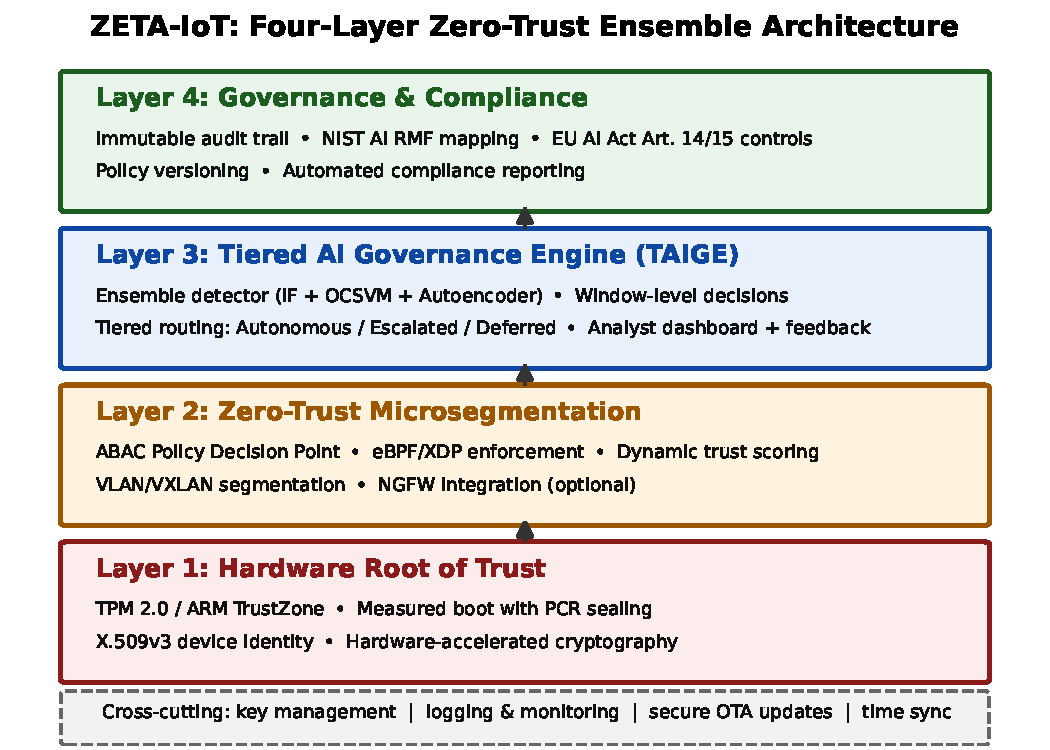
\includegraphics[width=\linewidth]{figures/fig_architecture.pdf}
  \caption{The ZETA-IoT four-layer architecture. Quantitative results in this paper validate the detection and routing functions of Layer~3; Layers~1, 2, and 4 are design contributions with commodity implementation paths.}
  \label{fig:arch}
\end{figure}

\textbf{Layer 1 --- Hardware Root of Trust (HRoT).} Each device anchors its identity in a TPM~2.0 module or ARM TrustZone. At boot, measurements of each stage extend the platform configuration registers; an X.509v3 identity certificate is bound to the TPM endorsement key; if measurements drift from the golden values, the device is quarantined. Commodity TPM modules cost on the order of tens of US dollars, keeping this layer viable for gateway-class devices.

\textbf{Layer 2 --- Zero-Trust Microsegmentation (ZTM).} Access decisions live on the gateway. An attribute-based access control (ABAC) engine weighs what it knows about a device (boot measurements, certificate validity, firmware version) together with a dynamic trust score, and enforcement happens in the kernel through eBPF/XDP packet filtering, fast enough for sub-millisecond decisions. Segmentation uses VLAN/VXLAN overlays, and enterprise firewalls can be integrated northbound where they exist. Because trust scores are pre-computed and policies compiled to kernel programs, no per-packet cloud round trip is required.

\textbf{Layer 3 --- Tiered AI Governance Engine (TAIGE).} The detection component is a lightweight ensemble of three one-class detectors, selected to span the three classical unsupervised paradigms and therefore three different failure modes: an Isolation Forest~\cite{liu2008iforest} (\emph{partitioning}: anomalies are isolated by random splits after fewer partitions than benign points), a one-class SVM~\cite{scholkopf2001ocsvm} trained via SGD on a Nystr\"om kernel approximation (\emph{boundary}: learns a hyperplane enclosing the benign cloud, sensitive to the geometry of the support region), and a fully connected autoencoder (\emph{reconstruction}: flags inputs it cannot compress and reconstruct, sensitive to the benign manifold's shape). The choice was driven by complementarity, not individual accuracy---the autoencoder alone saturates aggregate AUC on this benchmark (Section~\ref{sec:ablation})---and by operational constraints: all three train in seconds on a single CPU core without labelled attacks, and all three are megabyte-scale. Scores are standardised against a benign validation split and fused; decisions are taken over short windows of consecutive traffic snapshots (Section~\ref{sec:method}). The routing component classifies each alarm into one of three tiers (autonomous, escalated, deferred) under the decision contract of Section~\ref{sec:taige}.

\textbf{Layer 4 --- Governance \& Compliance (GCL).} Every decision, score, threshold, and human intervention lands in an append-only audit log. A compliance monitor then translates this operational record into regulatory language, as a design mapping: escalations to a human demonstrate the mechanism by which Article 14 oversight would be provided; the ensemble design and its measured false-positive behaviour speak to Article 15 robustness as an engineering target; score provenance in the audit trail provides transparency; and the same events map onto the AI RMF's Govern, Map, Measure, and Manage functions, whose voluntary status we do not imply otherwise~\cite{nistairmfvoluntary}. Mapped requirements are distinct from evidence of implementation or conformity, and Table~\ref{tab:spi} records which indicators are actually measured here. Policies, thresholds, and tier boundaries are kept as version-controlled configuration, so a governance decision is a reviewable artefact rather than a constant buried in code.

\subsection{Threat Model}
\label{sec:threat}

ZETA-IoT assumes an attacker who can reach the network segment an IoT device sits on, either by compromising the device itself (through default credentials, an unpatched service, or a supply-chain implant) or by joining the segment through a separate weakness such as a misconfigured access point. The attacker can send and receive arbitrary traffic on that segment and can attempt to blend malicious activity with the device's normal behaviour. Layer~3 detection is built for exactly this actor: Section~\ref{sec:results} evaluates it against real Mirai and BASHLITE infections, which is closer to this threat model than synthetic traffic replay.

Three capabilities are explicitly out of scope. First, an attacker who controls the hardware root of trust itself, for instance through physical access to the TPM or a supply-chain compromise of the boot chain, defeats Layer~1 by assumption; HRoT establishes a foundation to build on, not a defence against a fully compromised device. Second, an adaptive attacker who has access to the deployed models and deliberately crafts traffic to evade them is not evaluated here; the fusion design in Section~\ref{sec:ablation} is argued to raise the cost of evasion, but that argument is structural, not measured, and is listed as such in the limitations. Third, an attacker who can compromise the audit log or the policy configuration store directly bypasses Layer~4's guarantees; those guarantees assume standard access controls and integrity protection on the logging infrastructure, which this paper does not itself design or evaluate. Stating these boundaries is meant to make the security claims falsifiable rather than open-ended: the paper claims robustness against traffic-level evasion by volumetric botnets, not against an attacker who already owns the trust anchor.

\section{Tiered AI Governance Engine}
\label{sec:taige}

TAIGE operationalises AI--human complementarity through the decision taxonomy in Table~\ref{tab:tiers} and the decision contract in Figure~\ref{fig:contract}. The design premise is that governance requirements attach to \emph{decisions}, not to models: low-stakes, high-severity alarms can be acted on autonomously with post-hoc auditability, while high-stakes decisions require a human regardless of model output. One semantic distinction matters throughout: the thresholds $\theta_w$ and $\theta_{hi}$ are \emph{severity} calibrations---percentiles of benign validation scores, so they control the benign false-alarm rate and say nothing about the probability that a given alarm is an attack. \emph{Decision confidence} is a separate governance construct: it is the tier assignment itself (which procedures an alarm triggers), not a posterior probability. Conflating benign-tail rarity with attack probability would be a category error, and the contract below never interprets a percentile as a likelihood.

\begin{table}[t]
\caption{TAIGE decision tiers. $z$ is the fused window anomaly score; $\theta_w$ and $\theta_{hi}$ are the window alarm and high-severity thresholds calibrated on benign validation data (99th/99.9th percentiles). Stakes classes are policy-assigned per device. Critical-stakes devices are never acted on autonomously, at any severity: precedence rule~R1 in Figure~\ref{fig:contract}.}
\label{tab:tiers}
\small
\begin{tabular}{@{}llll@{}}
\toprule
Tier & Trigger & Action & Oversight \\
\midrule
Allow & $z \le \theta_w$ & forward & audit log \\
Autonomous & $z \ge \theta_{hi}$, low stakes & block/quarantine & post-hoc audit \\
Escalated & $\theta_w < z < \theta_{hi}$ (any stakes), or $z \ge \theta_{hi}$ on medium stakes & default action after 30\,s override window & analyst override within 30\,s \\
Deferred & $z > 3\theta_{hi}$ on critical device & recommend only; no autonomous act & human decides (SLA-bound) \\
\bottomrule
\end{tabular}
\end{table}

Precedence resolves the interaction the table cannot show in two columns. \textbf{R1 (critical precedence):} a critical-stakes device is never quarantined or blocked autonomously; any alarm above $\theta_w$ escalates to a human, with at most a \emph{restrictive interim action} (rate limiting to a policy floor, logging) that cannot take the device out of service. \textbf{R2 (override default):} every escalated alarm carries a stated default action; if no analyst responds within the 30\,s override window, the default action is applied automatically and the event is logged as \emph{autonomous-after-timeout}, with the analyst queue still holding it. On medium stakes the default is restrictive (throttle); on critical stakes it remains non-disruptive (throttle and re-alert, never quarantine). \textbf{R3 (analyst unavailability):} if no analyst acknowledges within the escalation SLA $T_{sla}$ (a policy value, e.g.\ 5\,min), the system executes the safety-limited default, flags the coverage gap in the audit log, and pages the next tier; escalation queues never silently drop an alarm. \textbf{R4 (deferral timeout):} a deferred recommendation that receives no human decision within $T_{sla}$ expires into the same safety-limited default (restrict, notify, re-alert); it never converts into a disruptive action.

\begin{figure}[t]
\centering
\begin{minipage}{0.96\linewidth}
\ttfamily\small
\raggedright
\textbf{on alarm}(device $d$, window score $z$)\\
\hspace*{1em}log$(d, z,$ all component scores, thresholds, feature summary$)$\\
\hspace*{1em}\textbf{if} $z \le \theta_w$: allow($d$); \textbf{return}\\
\hspace*{1em}$s \leftarrow$ stakes($d$) \hfill // policy-assigned: low / medium / critical\\
\hspace*{1em}\textbf{if} $s =$ critical: \hfill // R1: never autonomous\\
\hspace*{2em}\textbf{if} $z > 3\theta_{hi}$: defer($d$) \hfill // recommend only\\
\hspace*{2em}\textbf{else}: escalate($d$, interim=throttle) \hfill // intermediate alarm\\
\hspace*{1em}\textbf{elif} $s =$ medium:\\
\hspace*{2em}\textbf{if} $z \ge \theta_{hi}$: escalate($d$, interim=throttle, default=throttle)\\
\hspace*{2em}\textbf{else}: escalate($d$, interim=none, default=allow-with-watch)\\
\hspace*{1em}\textbf{else}: \hfill // low stakes\\
\hspace*{2em}\textbf{if} $z \ge \theta_{hi}$: quarantine($d$); post-hoc audit \hfill // autonomous\\
\hspace*{2em}\textbf{else}: escalate($d$, interim=none, default=allow-with-watch)\\
\hspace*{1em}wait analyst decision up to 30\,s \hfill // R2\\
\hspace*{1em}\textbf{if} no response: apply default; log(autonomous-after-timeout) \hfill // R2\\
\hspace*{1em}\textbf{if} no acknowledgement within $T_{sla}$: safety-limited default; page next tier \hfill // R3, R4\\
\rule{0pt}{0pt}\\
\emph{Invariants: critical devices are never quarantined autonomously (R1);}\\
\emph{every non-allow outcome is logged with its tier and evidence.}
\end{minipage}
\caption{TAIGE decision contract. Precedence: R1 critical devices are never acted on autonomously; R2 every escalation has a stated default applied after the 30\,s override window; R3 unacknowledged escalations execute a safety-limited default and page onward; R4 deferred recommendations expire into a safety-limited default, never a disruptive act. $\theta_w$, $\theta_{hi}$ are severity calibrations (benign-validation percentiles), not attack probabilities.}
\label{fig:contract}
\end{figure}

Escalated decisions surface to an analyst dashboard with the component scores, the fused score's position relative to calibrated thresholds, and the traffic features driving the alarm; analyst corrections feed back into threshold recalibration. The audit trail records which tier handled every event, satisfying the traceability expectations of NIST AI RMF's Govern function as a design mapping and providing the documentation basis that a conformity assessment under EU AI Act Article 14 would draw on. Tier boundaries, it should be stressed, are governance policy rather than learned parameters: an organisation can tighten $\theta_{hi}$ or reclassify device stakes without retraining.

\section{Evaluation Methodology}
\label{sec:method}

\subsection{Dataset}
The evaluation uses N-BaIoT~\cite{meidan2018nbaiot}, which captures real network traffic from nine commercial IoT devices (two doorbells, a thermostat, a baby monitor, four security cameras, a webcam) in a lab where each device was genuinely infected with the Mirai and BASHLITE botnets. Each traffic snapshot is a 115-dimensional feature vector produced by the extractor described with the dataset: statistics such as packet-count weight, mean, standard deviation, and (for two-stream aggregations) radius, magnitude, covariance, and correlation are computed over five stream aggregations, namely traffic from the source IP, from the source MAC-IP pair, the channel between source and destination IP, that channel's jitter, and the socket between source and destination IP:port, each tracked over five damped decay windows of progressively longer memory (100\,ms to 60\,s). The result is a snapshot that summarises both the immediate and the recent-minute behaviour of a flow in one vector, which is why a single reconstruction or partitioning model can separate a botnet's traffic pattern from a device's baseline without hand-engineered attack signatures. Seven devices have ten attack captures (five Mirai: \emph{ack, scan, syn, udp, udpplain}; five BASHLITE: \emph{combo, junk, scan, tcp, udp}); two devices, a doorbell and a webcam, have the five BASHLITE captures only, reflecting how the original data collection was carried out rather than any property of the detector evaluated here. For tractability, every capture is subsampled to at most 15{,}000 snapshots (per device and attack type; benign captures included), totalling $\approx$1.3M snapshots. The two capture types are subsampled differently, and we state both exactly: \emph{attack} captures with more than 15{,}000 snapshots are reduced by even systematic striding (every $\lfloor n/15000 \rfloor$-th row), which preserves capture-internal order at stride granularity; \emph{benign} captures are reduced by a seeded (RandomState 42) uniform random draw without replacement, which does not. The consequences for temporal interpretation are spelled out in Section~\ref{sec:protocol} rather than glossed over.

\subsection{Protocol}
\label{sec:protocol}
The protocol is designed to avoid the validation pitfalls catalogued by Arp et al.~\cite{arp2022dodo}, and it is reported here to the level of the exact operation order, so that no essential detail depends on the artifact alone:

\begin{enumerate}
\item \textbf{Per-capture subsampling.} For each device, each capture with more than 15{,}000 snapshots is reduced to 15{,}000: attack captures by even systematic striding (every $\lfloor n/15000 \rfloor$-th row of the stored capture, preserving capture-internal order at stride granularity), benign captures by a seeded (RandomState 42) uniform random draw without replacement (destroying capture-internal order). Stored order within each capture is otherwise the order produced by the extractor.
\item \textbf{Benign split.} For each device, the benign pool is \emph{shuffled} (RandomState 42) and split contiguously 60/20/20 into train, validation, and test. \emph{The split is not chronological.} The three detectors and the input scaler are trained on the training split only. No attack sample influences training or thresholds, so every attack is novel at test time. Per-device baselines mirror the deployment model in which each gateway learns its own devices' behaviour. A control experiment confirmed that a baseline transferred across devices collapses (benign traffic from other devices is flagged at 47--99\%), which is consistent with N-BaIoT's per-device design~\cite{meidan2018nbaiot}.
\item \textbf{Score standardisation and fusion.} Component scores are $z$-standardised per component using benign-validation statistics (mean, standard deviation), and fused by taking the maximum, an any-detector-fires rule; the precise definitions and the guarantees this does and does not provide are given in Section~\ref{sec:ablation}. Learned weighting was rejected deliberately: fitting weights needs labelled attacks, which the benign-only threat model denies, and any weight below one lets a confident detector be outvoted. Mean fusion is retained in the development ablation for exactly that reason.
\item \textbf{Window-level decisions.} Within each split and each attack capture separately, snapshots are grouped into disjoint consecutive windows of $W{=}11$ in stored order; the window score is the median fused score, and partial windows are dropped, so every snapshot contributes to at most one decision and no window crosses a split or capture boundary. $W{=}11$ was fixed before any attack was scored: an odd window lets the median suppress up to five isolated benign outliers while sustained attack elevation survives, and it follows the window-voting evaluation philosophy of Meidan et al.~\cite{meidan2018nbaiot}, who optimised the window per device on benign data; we fix one value to keep the protocol device-independent. The development failure analysis in Section~\ref{sec:ablation} is separate: it motivated the fusion design but does not enter any reported number, which comes from the final converged models under this protocol.
\item \textbf{Threshold calibration.} The instance alarm threshold is the 99th percentile of benign validation instance scores, and the window alarm threshold $\theta_w$ the 99th percentile of benign validation window scores, targeting a 1\% false-positive rate without touching test data; the high-severity threshold $\theta_{hi}$ is the 99.9th percentile.
\end{enumerate}

\paragraph{Temporal status of the evaluation.} The evaluation is \emph{not} chronological, in two respects. First, the benign split is random: shuffling before splitting destroys any drift or regime structure, so all three splits see the same mixture of device behaviours. Second, window content differs by capture type: attack windows are built in capture order (strided but ordered), so sustained attacks stay sustained within a window, whereas benign test windows are built in the stored order of a random subsample of a shuffled split, so their snapshots need not be adjacent in wall-clock time. We therefore do \emph{not} interpret the results as a measurement of detection latency or of performance on drifting traffic. Two mitigations bound the damage. On the benign side, a chronological held-out check on the largest capture (Danmini doorbell, 49{,}548 snapshots) re-runs the full pipeline with the benign data kept in original capture order: the window-level false-positive rate is 0.67\% (vs.\ 1.66\% under the shuffled protocol; nominal target 1\%), so benign FPR does not degrade under temporal ordering on this device---if anything the shuffled protocol is conservative here. On the attack side, attack captures are separate files with no interleaved benign traffic, so a chronologically faithful attack TDR in a mixed stream would require live data; that is precisely what the pilot (Section~\ref{sec:discussion}) is for. As for the original-time span of a window: the public release carries no timestamps, snapshots are packet-triggered, and each snapshot's features already aggregate up to 60\,s of traffic history, so a window's wall-clock footprint is at most the inter-snapshot gaps of its 11 stored-order snapshots plus the 60\,s feature tail; the exact span is not recoverable from the public files and we make no claim about it.

\subsection{SPI Framework}
The framework tracks 14 Security Performance Indicators in four groups. Five cover detection: detection rate, false positives, latency, adversarial evasion, and performance on novel attacks (SPI-1 to SPI-5). Four cover resilience under attack: uptime, recovery time, service degradation, and containment (SPI-6 to SPI-9). Four more concern governance: escalation accuracy, human override rate, compliance coverage, and audit completeness (SPI-10 to SPI-13). The last, SPI-14, is the resource budget: CPU, memory, and model footprint. Table~\ref{tab:spi} records which of these the present evaluation can support. Five are measured in full: SPI-1, SPI-2, and SPI-5 (every attack is unseen by construction), together with the scoring-latency component of SPI-3 and the resource budget SPI-14. Two are partial: for SPI-10, the routing distribution is measured but escalation \emph{correctness} is not, since judging whether an escalation was warranted requires an analyst; for SPI-13, the audit-log mechanism runs and is measured, but its completeness has not been independently verified. The remaining seven indicators require a live deployment with human analysts and attack campaigns against running infrastructure; they are defined here as the measurement plan for a future pilot and are deliberately \emph{not} estimated synthetically.

Defining an indicator before it can be measured is deliberate. Recovery time (SPI-7) only means something once there is a real containment action to time, and human override rate (SPI-11) only means something once real analysts are making real overrides; a plausible-sounding number for either without that context is the kind of unfalsifiable claim Section~\ref{sec:introduction} argues against. Fixing the success criteria now, before the pilot's data exists, is meant to stop them being chosen afterward to flatter the results.

\begin{table}[t]
\caption{Security Performance Indicator (SPI) measurement status. $\bullet$ = measured here; $\circ$ = defined but deferred to the live pilot; \emph{partial} = mechanism measured, human-judgement component deferred. Deferred items require analysts in the loop or attacks against running infrastructure, neither of which a public traffic dataset can supply.}
\label{tab:spi}
\small
\begin{tabular}{@{}clcc@{}}
\toprule
SPI & Indicator & Status & Section \\
\midrule
1 & Detection rate (TDR) & $\bullet$ & \ref{sec:results} \\
2 & False-positive rate & $\bullet$ & \ref{sec:results} \\
3 & Latency & $\bullet$ (x86, single-model) & \ref{sec:results} \\
4 & Adversarial evasion & $\circ$ & future pilot \\
5 & Novel-attack detection & $\bullet$ & \ref{sec:results} \\
6--9 & Resilience indicators & $\circ$ & future pilot \\
10 & Escalation accuracy & partial & \ref{sec:results} \\
11 & Human override rate & $\circ$ & future pilot \\
12 & Compliance coverage & $\circ$ & future pilot \\
13 & Audit completeness & partial & \ref{sec:results} \\
14 & Resource budget & $\bullet$ (x86, serialized size) & \ref{sec:results} \\
\bottomrule
\end{tabular}
\end{table}

\subsection{Implementation}
Everything is built on scikit-learn~\cite{sklearn}. The Isolation Forest uses 200 trees with a subsample of 1024; the one-class SVM is trained with SGD on a 100-component Nystr\"om approximation ($\nu{=}0.05$); the autoencoder is a 48--8--48 network trained for 120 epochs. All timings come from a single x86-64 CPU core in a containerised Linux environment; the specific CPU model and peak resident memory are not recorded and we make no claim about them. They should be read as commodity-CPU indications; profiling on ARM gateways belongs to the pilot. Code, configuration, and per-device result files are provided in the anonymized artifact repository (\url{https://anonymous.4open.science/r/zeta-iot-artifact-42B3}), together with the scripts that produced every table and figure.

\subsection{Reproducibility}
Every stage is deterministic given a fixed random seed (42 throughout: benign subsampling, shuffling, splits, model initialisation; the attack-cap striding is deterministic), so re-running the released scripts against the public N-BaIoT release reproduces Tables~\ref{tab:overall} and~\ref{tab:ablation} exactly. Data preparation, training, evaluation, and figure generation are separate scripts with intermediate output written to disk, so a reviewer can re-run only the evaluation stage against the provided checkpoints, or the full pipeline from raw data. No result depends on a split chosen after seeing the outcome: splits, thresholds, the window length, and tier boundaries are fixed by the protocol in Section~\ref{sec:protocol} before any attack data is scored. All protocol details needed to interpret the results appear in this paper; the artifact adds runnable code, not missing facts.

\section{Results}
\label{sec:results}

\subsection{Detection Performance}
\label{sec:detection}

Table~\ref{tab:overall} summarises aggregate results over all nine devices (104{,}347 attack windows, 2{,}414 benign test windows). At window level the ensemble detects \textbf{100\% of attack windows for every one of the ten attack types on every device}, at an aggregate false-positive rate of 1.45\% (per-device range 0--2.6\%) and macro-averaged AUC of 0.9996. Because training saw no attack data, this is novel-attack detection by construction (SPI-5).

\begin{table}[t]
\caption{Aggregate detection results across nine devices. Instance = per-snapshot decisions; Window = median over $W{=}11$ stored-order snapshots. Thresholds fixed at the 99th percentile of benign validation scores.}
\label{tab:overall}
\small
\begin{tabular}{@{}lcc@{}}
\toprule
Metric & Instance-level & Window-level \\
\midrule
Detection rate (TDR, SPI-1) & 80.1\% & \textbf{100.0\%} \\
False-positive rate (SPI-2) & 0.93\% & 1.45\% \\
Macro AUC & --- & 0.9996 \\
Mirai TDR & 99.98\% & 100.0\% \\
BASHLITE TDR & 64.4\% & 100.0\% \\
\bottomrule
\end{tabular}
\end{table}

Figure~\ref{fig:perattack} breaks the results down by attack type, and the instance/window contrast is instructive---it also explains the otherwise surprising pattern behind the saturated headline. Eight of the ten attack types are detected at $\ge$99.8\% even at instance level, because volumetric botnet traffic sits orders of magnitude away from benign behaviour on these features. The two exceptions, BASHLITE \emph{tcp} and \emph{udp}, are detected on only one device class at instance level (11\% mean TDR) even though their scores sit far above the benign median; on the worst device their reconstruction error is $37\times$ the benign median. The reason is the threshold, not the models: benign validation scores have heavy tails, and a handful of legitimate traffic bursts push the 99th-percentile line above the attack scores. Window-median smoothing collapses that tail while sustained attacks stay elevated, lifting these attacks to 100\% with no change to models or training. The 100\% window-level rates are therefore a joint property of the benchmark's attack separation and the window rule, not evidence that ten distinct attack families were each individually hard.

Uniform window-level detection deserves a caveat and an explanation. It is a property of this benchmark as much as of the detector: N-BaIoT's botnet traffic is volumetric and statistically far from benign behaviour, and the dataset's authors likewise reported near-complete detection with per-device models~\cite{meidan2018nbaiot}. The informative quantity once detection saturates is the \emph{margin} by which attacks clear the alarm threshold, shown in Figure~\ref{fig:margins}. Margins vary across attack types by four orders of magnitude, and the tcp/udp floods survive by a factor below two. That is a reminder that a modest adversarial shift could push such attacks under the line, which is why the fusion and windowing choices in Sections~\ref{sec:protocol} and~\ref{sec:ablation} matter more than the headline rate. Per-device FPR and AUC are shown in Figure~\ref{fig:perdevice}; the lowest per-device AUC is 0.997.

\begin{figure}[t]
  \centering
  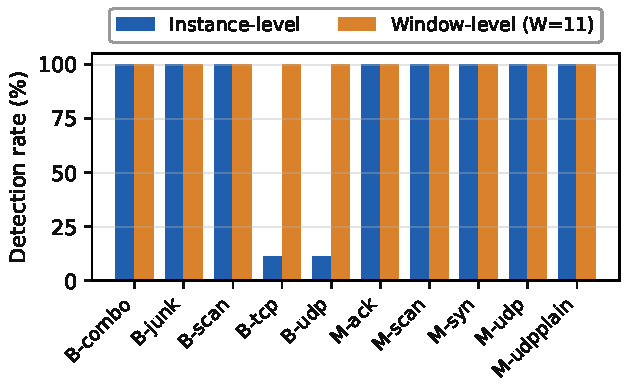
\includegraphics[width=\linewidth]{figures/fig_per_attack.pdf}
  \caption{Detection rate by attack type (M- = Mirai, B- = BASHLITE), mean across devices. Eight of ten attacks exceed 99.8\% at instance level; the two BASHLITE floods fail only at instance level (benign heavy tails lift the threshold above moderate attack scores) and are recovered entirely by window-median decisions.}
  \label{fig:perattack}
\end{figure}

\begin{figure}[t]
  \centering
  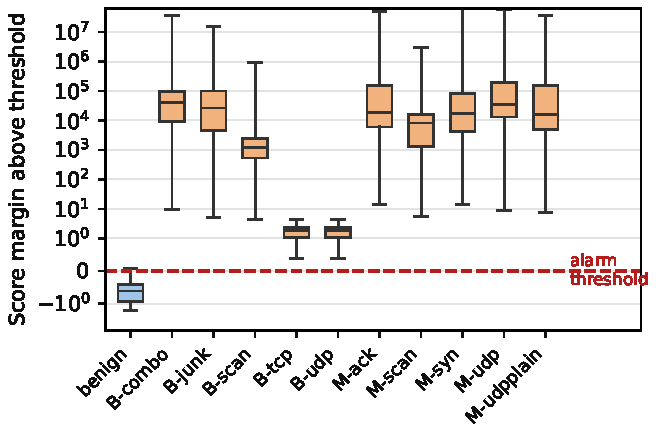
\includegraphics[width=\linewidth]{figures/fig_score_margins.pdf}
  \caption{Distribution of window-median anomaly scores relative to each device's calibrated alarm threshold, pooled over devices. The plotted ordinate is the transformation $r = \log_{10}(z_w / \theta_w)$, so the dashed line at $r{=}0$ marks $z_w = \theta_w$ and a value of $r$ is read as a multiplicative margin: the whiskers span the 1st--99th percentiles of $r$. Detection saturates because every attack window scores above threshold, but the margins differ by orders of magnitude: most botnet traffic clears the line by $10^3$--$10^5$, while the BASHLITE tcp/udp floods pass it by a factor below two. The margin is a property of scores and thresholds; it is not, by itself, a measure of the size of an adversarial traffic perturbation.}
  \label{fig:margins}
\end{figure}

\begin{figure}[t]
  \centering
  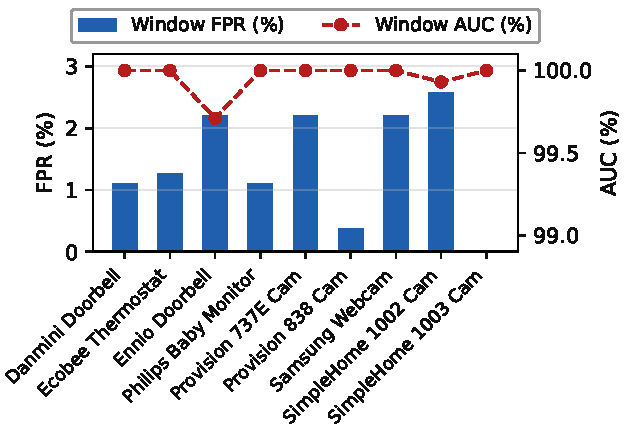
\includegraphics[width=\linewidth]{figures/fig_per_device.pdf}
  \caption{Window-level false-positive rate and AUC per device.}
  \label{fig:perdevice}
\end{figure}

\subsection{Ablation: What the Ensemble Does and Does Not Guarantee}
\label{sec:ablation}

\paragraph{Score and threshold definitions.} For a snapshot $x$, the three component scores are $s_{\mathrm{IF}}(x) = -f_{\mathrm{IF}}(x)$ and $s_{\mathrm{SVM}}(x) = -f_{\mathrm{SVM}}(x)$ (negated decision functions, higher = more anomalous) and $s_{\mathrm{AE}}(x) = \mathrm{MSE}(x, \hat{x})$. Standardisation uses benign validation statistics: $z_j(x) = (s_j(x) - \mu_j)/\sigma_j$. The fused score is $z(x) = \max_j z_j(x)$, and a window alarms when its median fused score exceeds $\theta_w = Q_{0.99}(\text{benign validation window scores})$; $\theta_{hi} = Q_{0.999}$ of the same distribution.

\paragraph{What max fusion guarantees.} Because the maximum is order-preserving, for \emph{any} common threshold $\tau$,
\[
z(x) \ge \tau \iff \exists j:\; z_j(x) \ge \tau .
\]
Two consequences follow exactly. (i) Every alarm of the fused rule at $\tau$ is witnessed by at least one component at the same standardised level $\tau$; the fused rule cannot fire on a coalition of sub-threshold components, which is precisely the failure that mean fusion exhibited in development (below). (ii) Evasion of the fused rule at $\tau$ requires keeping \emph{every} component below $\tau$---an attacker must fool all three detectors at the fused operating point, not just the weakest one.

\paragraph{What it does not guarantee.} The earlier framing---that an attack ``must evade every detector's calibrated threshold at once''---conflated the common threshold $\tau$ with each detector's separately calibrated threshold $\theta_j = Q_{0.99}(z_j$ on validation$)$. Since $\max_j z_j \ge z_j$ pointwise, the 99th percentile of the fused distribution satisfies $\theta_w \ge \theta_j$ for every component, with equality only under perfect correlation. A component can therefore exceed its own calibrated threshold $\theta_j$ while the fused score remains below $\theta_w$; individually calibrated per-detector alarms can be absorbed by fusion. ZETA-IoT's operational rule is a \emph{single} alarm line at $\theta_w$---not three autonomous per-detector lines---so this absorption is a deliberate simplification of the alert surface, and per-detector exceedances serve as analyst diagnostics rather than autonomous triggers. We correct the guarantee accordingly: evasion requires all components below $\theta_w$; it does \emph{not} require all components below their own $\theta_j$.

\paragraph{Evidence.} Table~\ref{tab:ablation} reports window-level AUC per component and for the max-fused ensemble. The ensemble does not improve aggregate discrimination---the autoencoder alone reaches 1.0000 against the ensemble's 0.9996---and we do not claim that it does. The case for the ensemble is robustness to single-detector failure modes, and it rests on two pieces of evidence. First, the development failure analysis: an undertrained autoencoder assigned benign-level reconstruction error to BASHLITE floods that the Isolation Forest scored at $z \approx 3.6$, and mean fusion diluted the alarm below threshold---one detector's catch was silently outvoted. Max fusion removes this failure mode structurally, at the cost of three score evaluations per snapshot instead of one. Second, the structural argument of the previous paragraph: at the fused operating point, an adaptive attacker must depress all three components below $\theta_w$, so a single-detector blind spot does not by itself open an evasion path. This is a design-time argument about the alarm rule; it is not a measured adversarial-robustness claim, and adaptive-attack evaluation remains deferred (SPI-4). At matched false-positive budgets, the relevant operating-point quantities---component TDR, fusion TDR, scoring cost, and missed-attack overlap between fusion rules---are computed from saved per-window scores by the released script \texttt{matched\_fpr.py}; the aggregate-AUC comparison in Table~\ref{tab:ablation} already shows why the ensemble's justification is robustness rather than discrimination.

\begin{table}[t]
\caption{Window-level AUC by ensemble component (mean over devices). The ensemble does not improve aggregate AUC; its justification is robustness to single-detector failure modes (Section~\ref{sec:ablation}).}
\label{tab:ablation}
\small
\begin{tabular}{@{}lcccc@{}}
\toprule
 & IF & OCSVM & AE & Ensemble (max) \\
\midrule
AUC & 0.9983 & 0.9994 & 1.0000 & 0.9996 \\
\bottomrule
\end{tabular}
\end{table}

\subsection{Resource Footprint}
\label{sec:resources}

The mean per-device ensemble occupies \textbf{3.6\,MB} of \emph{serialized} (pickled) storage and trains in 11.1\,s on a single commodity x86 CPU core, so retraining a device baseline is an online operation rather than an offline batch job. Scoring one snapshot through all three detectors of one device takes 16.4\,ms single-sample, but 0.022\,ms per snapshot when scored in a batch of 4{,}096 through that same device's models (SPI-3/14, x86 indication). We state the measured workload exactly: the batch figure is a 4{,}096-snapshot batch through \emph{one} device's ensemble, not a mixture of models across devices. Because Section~\ref{sec:protocol} trains a distinct model set per device, this measurement supports a per-device throughput claim---roughly 45{,}000 snapshots per second per device model on one core---and no more: cross-model dispatch, batch waiting time under a multi-device arrival process, and peak resident memory were not measured, and we do not extrapolate the single-model batch figure into a gateway-wide capacity claim. A gateway serving $D$ devices holds $D$ ensembles ($3.6\,\mathrm{MB} \times D$ serialized) and must either timeshare cores or schedule models; that scheduling benchmark, together with ARM-native scoring and on-gateway feature extraction, belongs to the planned pilot. The serialized 3.6\,MB is a storage figure, not a runtime memory budget.

\subsection{Decision Routing Analysis}
\label{sec:routing}

To exercise TAIGE's routing on real scores rather than synthetic ones, all test windows were replayed through the decision contract of Figure~\ref{fig:contract} under an illustrative policy (cameras, doorbells, and monitors classed as elevated stakes; all other devices low stakes). Of 106{,}761 windows: 2.2\% were allowed (benign below threshold; 98.6\% of benign windows), 11.8\% were handled autonomously, 12.8\% escalated, and 73.2\% deferred. That deferral figure is an artefact of composition, not of policy aggressiveness: attack windows outnumber benign ones 43:1 in the test set, whereas production traffic is overwhelmingly benign. The per-class rates are what the policy actually fixes: benign windows route 98.6\% allow and 1.4\% escalate, attack windows 74.9\% defer, 13.1\% escalate, and 12.1\% autonomous, with no attack window ever allowed. Because those per-class rates are fixed, the operational load under any traffic mix can be obtained by reweighting them. At 1\% attack prevalence the same thresholds yield 0.8\% deferred and 1.6\% escalated; at 0.1\% prevalence, 0.1\% and 1.5\%. Analyst workload is therefore governed by the benign false-positive rate, not by the deferral share seen in this attack-saturated test set.

Two clarifications bound this analysis. First, it demonstrates the routing \emph{mechanism} and its auditability---every window carries its tier assignment in the results artefact---not the safety or efficacy of the interventions themselves, which require the live pilot. Second, the safety-relevant boundary cases of the contract behave as specified: an intermediate-score alarm on a critical device escalates rather than acting autonomously (precedence R1), an unacknowledged escalation executes its stated restrictive default after the override window (R2), and a deferred recommendation on a critical device never converts into a disruptive act (R4). Calibrating tier boundaries against analyst capacity, and measuring escalation accuracy and override rates (SPI-10/11), requires the live pilot.

\section{Discussion}
\label{sec:discussion}

\textbf{Mapping results to the architecture.} Each measured result validates a specific architectural function, and we keep the mapping explicit. The detection results (Tables~\ref{tab:overall} and~\ref{tab:ablation}, Figures~\ref{fig:perattack}--\ref{fig:perdevice}) validate Layer~3's detection core under the benign-only protocol. The routing analysis (Section~\ref{sec:routing}) validates Layer~3's decision routing and audit trail on real scores. The resource measurements (Section~\ref{sec:resources}) provide the feasibility evidence that Layer~2's gateway-resident intelligence requires: per-device scoring fits in milliseconds and megabytes on a commodity core. Layers~1, 2, and 4 remain design contributions with cited implementation paths; nothing in this paper claims an integrated four-layer deployment.

\textbf{Architectural fragmentation (G1).} The architecture demonstrates that the detection layer of a zero-trust IoT design fits within megabyte and millisecond budgets on commodity CPUs, addressing the primary feasibility concern for gateway-resident intelligence. The remaining layers compose from commodity mechanisms (TPM~2.0, eBPF/XDP, ABAC engines) whose individual feasibility is established; their integrated evaluation is future work.

\textbf{Governance disconnect (G2).} The tiered taxonomy shows one concrete way to make ``human-in-the-loop'' operational: attach oversight requirements to decision stakes and score severity rather than to the model, calibrate thresholds on benign data, make tier boundaries versioned policy, and give every escalation a stated default for the no-analyst case. The routing analysis confirms the mechanism produces auditable, policy-sensitive distributions on real detection output, and the contract of Figure~\ref{fig:contract} closes the cases a table cannot: critical devices are never acted on autonomously, and unanswered escalations degrade to safety-limited defaults rather than to silence or to full autonomy.

\textbf{Validation realism (G3).} Benign-only per-device ensembles detect all ten real botnet attack types completely at window level with FPR under 2.6\% per device. Three methodological findings generalise beyond this paper: (i) cross-device baseline transfer fails catastrophically, so architectures must budget for per-device (or per-class) learning; (ii) threshold placement and score fusion, not model capacity, were the binding constraints on detection, and both are correctable with governance-level configuration rather than retraining; (iii) the evaluation's non-chronological protocol (Section~\ref{sec:protocol}) is defensible for FPR---the chronological held-out check shows no degradation---but temporal claims about detection latency and drift await the pilot.

\textbf{Comparison with prior detection work.} We restate the comparison with verified facts. Meidan et al.~\cite{meidan2018nbaiot} train per-device autoencoders on benign-only data with chronological splits and report near-complete detection on this dataset; our window-level results are consistent with theirs rather than an improvement, and our autoencoder component alone matches their detector family. Our contribution relative to that line is the ensemble across complementary detector families with an explicit margin analysis (Figure~\ref{fig:margins}), the corrected fusion analysis, and the governance architecture around the detector---not benign-only training (which we adopt from them), not a higher detection rate on a near-saturated benchmark, and not a smaller model (their per-device autoencoders are 172\,kB by object size; our serialized ensemble is 3.6\,MB). Diro and Chilamkurti's reported accuracy comes from NSL-KDD and BoT-IoT, benchmarks built around simulated or non-IoT traffic, so a number from that setting and a number from genuinely infected consumer devices are not measuring the same thing and no ranking is claimed between them.

\textbf{Practical implications.} Three points follow for anyone deploying this design rather than reading about it. Per-device models mean per-device overhead: fifty endpoints need fifty small ensembles, and the 11.1-second training time in Section~\ref{sec:resources} makes retraining manageable but not free when a device or its firmware changes. The threshold is a safety-relevant configuration value, not a set-once hyperparameter; benign traffic drifts, so recalibration against fresh data should be routine, not a one-time step at deployment---and because benign-tail percentiles control false-alarm rate rather than attack probability, drift monitoring belongs on the score distribution, not on the alarm count alone. And the governance layer only delivers the compliance evidence Section~\ref{sec:taige} describes if the audit log itself is protected and retained, so Layer~4 should be treated as a specification to implement and secure, not a feature that arrives automatically once Layer~3 is running.

\textbf{Limitations.} Each limitation is tied to what was and was not measured. First, the empirical claims cover Layer~3 only; Layers~1/2/4 are designs with cited implementation paths, and end-to-end evaluation on physical gateways (including ARM latency, TPM boot-time, and eBPF throughput measurements) is planned. Second, the evaluation is not chronological (Section~\ref{sec:protocol}); the benign FPR side is covered by a chronological held-out check on one device, but attack-side temporal detection and any drift behaviour require the pilot. Third, N-BaIoT's 115 features are pre-extracted; on-gateway feature computation cost is not measured here. Fourth, the resource figures are single-model x86 measurements (Section~\ref{sec:resources}); multi-device scheduling, peak memory, and the specific CPU model are unreported, and the 3.6\,MB figure is serialized storage. Fifth, the dataset covers two botnet families on nine consumer devices; industrial protocols and slow, stealthy attacks (as opposed to volumetric botnet traffic) are open questions. Window-median smoothing that helps against floods could equally delay detection of a low-rate attack that never produces a sustained spike. Sixth, adversarial evasion (SPI-4) is argued structurally via fusion design (Section~\ref{sec:ablation}) but not yet measured against adaptive attackers~\cite{alhajjar2021}. Seventh, governance indicators involving humans (SPI-10/11) await the pilot. These bounds are stated explicitly in the spirit of~\cite{arp2022dodo}, on the view that a security paper which cannot say what it has not tested is not making a security claim at all.

\textbf{Future work.} The most immediate step is the live pilot referenced throughout this paper, since it is the only way to measure SPI-10 through SPI-12 honestly rather than assume them. Three further extensions matter independently of the pilot: evaluating against an adaptive attacker to turn the structural evasion argument in Section~\ref{sec:ablation} into a measured one, extending beyond N-BaIoT's feature space to industrial protocols such as Modbus/TCP, and replacing fixed percentile thresholds with an adapting baseline, provided the adaptation itself remains auditable rather than becoming a second black box inside Layer~3.

\section{Conclusion}
ZETA-IoT brings zero-trust principles, resource-frugal ensemble detection, tiered AI--human governance, and compliance mapping together in a single architecture for IoT edge security. Its detection layer, validated reproducibly on real botnet traffic from nine commercial devices under a strict benign-only protocol with an exactly specified operation order, achieves complete window-level detection of all ten attack types at a 1.45\% false-positive rate within a 3.6\,MB serialized footprint per device. Serious IoT security intelligence, in other words, does not require server-class resources, though the margin analysis in Section~\ref{sec:results} is a reminder that a saturated detection rate is not the same thing as a comfortable safety margin.

The tiered governance engine, its complete decision contract, and the SPI framework provide an operational bridge from NIST AI RMF and EU AI Act obligations to millisecond-scale security decisions, with the indicators that require humans honestly deferred to a live pilot rather than simulated. That honesty is itself part of the argument this paper is making: a governance mechanism whose evidence is manufactured to fit its own claims is not a governance mechanism, whatever else it might be. Whether ZETA-IoT's specific tier boundaries and thresholds are the right ones for a given deployment is an empirical question the pilot is designed to answer; what this paper claims is narrower and, it hopes, more durable, namely that detection, routing, and audit can be built as one architecture on hardware an ordinary IoT gateway already has. Code and evaluation artefacts are available in anonymized form at \url{https://anonymous.4open.science/r/zeta-iot-artifact-42B3} to support replication and, ideally, to let that claim be checked independently rather than taken on trust.

% Acknowledgments omitted for anonymous review

\bibliographystyle{ACM-Reference-Format}
\bibliography{refs}

\end{document}
